\documentclass[exercice]{thedocument}%
\startdatakeys
\source{}
\BO{2026}
\cycle{4}
\competencesDuSocle{CA}
\objectifsApprentissage{A1aa}
\automatismes{}
\enddatakeys
\begin{document}%
% \begin{center}\pdf[scale=0.75]{Cycle4-Myriade-50-3}\end{center}
Dans la figure ci-dessous, \mathspoint{ABCD} et \mathspoint{EFGC}
sont des rectangles.
\begin{center}
    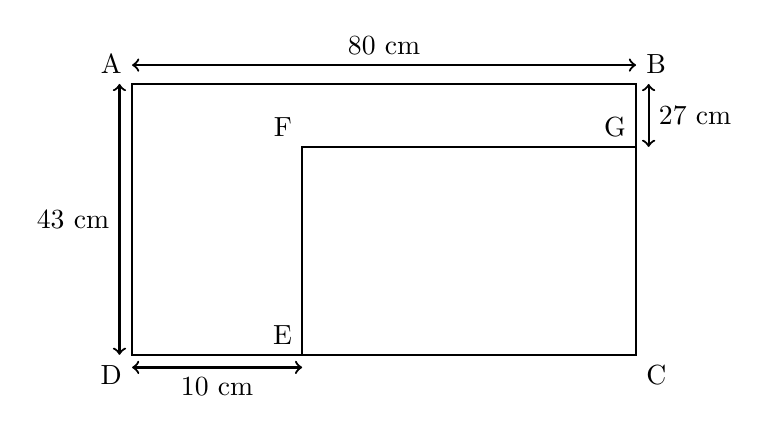
\begin{tikzpicture}[line width=0.8pt, scale=0.8]
        \coordinate[label=above left:\mathspoint{A}](A)at(0,4.3);
        \coordinate[label=below left:\mathspoint{D}](D)at(0,0);
        \coordinate[label=above right:\mathspoint{B}](B)at(8,4.3);
        \coordinate[label=below right:\mathspoint{C}](C)at(8,0);
        \coordinate[label=above left:\mathspoint{E}](E)at(2.7,0);
        \coordinate[label=above left:\mathspoint{F}](F)at(2.7,3.3);
        \coordinate[label=above left:\mathspoint{G}](G)at(8,3.3);
        \draw(A)--(B)--(C)--(D)--cycle;
        \draw(E)--(F)--(G);
        % Cote AB
        \draw[<->] (0,4.6) -- node[above] {80 cm} (8,4.6);

        % Cote BG
        \draw[<->] (8.2,3.3) -- node[right] {27 cm} (8.2,4.3);

        % Cote DE
        \draw[<->] (0,-0.2) -- node[below] {10 cm} (2.7,-0.2);

        % Cote AD
        \draw[<->] (-0.2,0) -- node[left] {43 cm} (-0.2,4.3);
    \end{tikzpicture}
\end{center}
\begin{enumerate}
    \item Écrire une expression qui permet de calculer l'aire
    du rectangle \mathspoint{EFGC}.
    \item Écrire une expression qui permet de calculer le
    périmètre du rectangle \mathspoint{EFGC}.
    \item Calculer l'aire et le périmètre du rectangle
    \mathspoint{EFGC}. 
\end{enumerate}
\end{document}
